\documentclass[conference]{IEEEtran}
\IEEEoverridecommandlockouts
% The preceding line is only needed to identify funding in the first footnote. If that is unneeded, please comment it out.
\usepackage{cite}
\usepackage{amsmath,amssymb,amsfonts}
\usepackage{algorithmic}
\usepackage{graphicx}
\usepackage{textcomp}
\usepackage{xcolor}
\usepackage{multirow}
\def\BibTeX{{\rm B\kern-.05em{\sc i\kern-.025em b}\kern-.08em
    T\kern-.1667em\lower.7ex\hbox{E}\kern-.125emX}}
\begin{document}

\title{Comparing Reinforcement Learning and Finite State Machine Agents in Real Time Strategy Games: Impact on Player Experience}

\author{\IEEEauthorblockN{Joshua Polanszky}
	\IEEEauthorblockA{\textit{Institute of Information Communication Technology} \\
		\textit{Malta College of Arts Science and Technology}}
	Paola, Malta
}

\date{\today}

\maketitle

\begin{abstract}
	abstract
\end{abstract}

\begin{IEEEkeywords}
	Keywords
\end{IEEEkeywords}

\section{Introduction}

% Introduction Section. Example citations: \cite{ronneberger2015unet} and \cite{latex2e}

\subsection{Theme and Topic Rationale}

The Theme chosen is Decision-Making AI for Real-Time Strategy (RTS) Games, and will focus on comparing Finite State-Machine (FSMs) AI opponents traditionally used in games, against Machine Learning (ML) opponents, specifically
Reinforcement Learning (RL), and their impact on player experience.

Game AI plays a huge role in player experience and immersion, as they provide the challenge and unpredictability that makes games fun and engaging.
While extensive research has been conducted on the topic, most have focused more on the pure performance of the RL agent, and/or its impact on player experience, never directly
comparing it to traditional FSMs, such as the work done by Grech \cite{grech_creating_2023}, Berta, et al. \cite{bin_ramlan_implementation_2021}, and Zhasulanov \cite{zhasulanov_enhancing_2024}.
This study aims to address the research gap by directly comparing RL Agents to FSMs, and evaluating their impact on player experience, with the goal of identifying if the computational
and development cost of implementing RL agents is justified by the improvement in player experience.

\subsection{Positioning and Research Onion}
This research addresses the gap in player experience found in the literature, building on the works of \cite{grech_creating_2023} and \cite{vinyals_grandmaster_2019} on AlphaStar by providing a better understanding on the role RL agents will play in the future of RTS games.
As can be seen in Figure \ref{fig:research_onion}, this study will follow a positivist research paradigm, following a deductive and experimental approach, gathering both quantitative and qualitative data to measure player experience.

\begin{figure}[htbp]
	\centering
	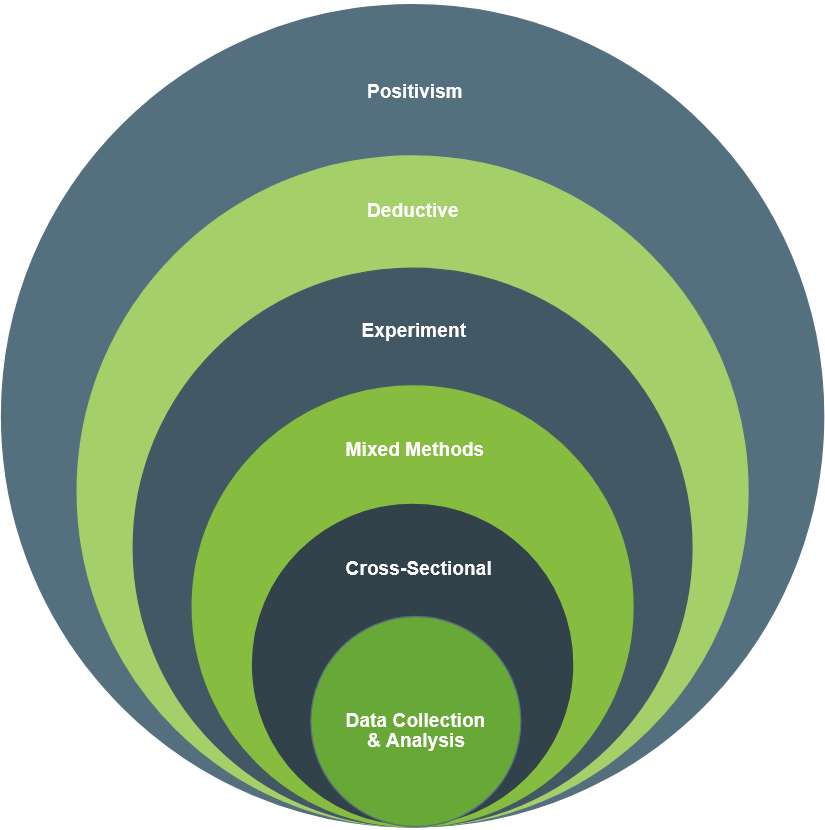
\includegraphics[width=0.45\textwidth]{../Images/Research_Onion.PNG}
	\caption{Research Onion}
	\label{fig:research_onion}
\end{figure}

\subsection{Background to the Research Theme}
Game AI has evolved significantly over the years, especially in RTS games. Early RTS titles, such as StarCraft, relied on Finite State Machines (FSMs) for their AI decision-making. These FSM-based approached
are deterministic and predictable, which can lead to repetitive and boring gameplay, and allow players to exploit the gameplay patters of the AI. \cite{vinyals_grandmaster_2019}

More recently, RL has emerged as an alternative AI approach, taking advantage of advancements in ML and computer hardware. In games such as AlphaStar \cite{vinyals_grandmaster_2019}, RL agents were able to
demonstrate adaptive and human-like behaviour, providing a more challenging and engaging experience for players. Another paper that highlights this is the work done by Grech \cite{grech_creating_2023},
where he created multiple difficulties of AI opponents using RL, and found that players reported higher levels of enjoyment and immersion. A similar study is the one done by \cite{bin_ramlan_implementation_2021},
where they trained an RL agent to act as an opponent in a fighting game, with the agent being able to adapt to the player's skill level, and provide a more engaging experience, similar to the work done by \cite{vinyals_grandmaster_2019}

Despite all of this, the implementation of RL in commercial games remains limited due to the high computational cost, long training and development times, and added complexity.
This further proves the need for research in this area, and in evaluating if the benefits of RL agents in RTS games are worth the cost compared to traditional FSMs.

\subsection{Hypothesis}

Players report a higher level of enjoyment and improved experience when playing against RL agents comparted to FSMs in RTS games.

\subsection{Independent \& Dependent Variables}

Independent variables are variables that are manipulated by the researcher, and are mainly used to influence the dependant variables. Dependant variables are what happen as a result of the independant variables,
and are what the researcher is interested in measuring.

The independent variable in this study is the type of AI opponent. The dependant variables, those are player experience, player immersion, and perceived difficulty.
Player experience will be measured through surveys and engagement metrics, player immersion will be measured through surveys and validated game design principles, and perceived difficulty will be measured through
surveys, player feedback, and engagement metrics.

\subsection{Research Aim}

The aim of this study is to evaluate the impact of Reinforcement Learning (RL) and Finite State Machines (FSMs) AI opponents on player experience in Real-Time Strategy (RTS) games, and determine if the extra resources
is justified by the improvement in player experience for RL agents.

To be more specific, the study will focus on the following research objectives:

\begin{itemize}
	\item Compare player-reported enjoyment and engagement levels when playing against RL and FSM AI opponents in RTS games.
	\item Assess the impact of RL and FSM AI opponents on player immersion in RTS games.
	\item Determine if the computational and development costs and complexity of RL justify its implementation over FSMs in RTS games.
\end{itemize}

\subsection{Purpose Statement}

This study is important because AI opponents shaoe the core gameplay experience of RTS games. While FSMs remain widely used due to their simplicity, RL-based AI has the potential to revolutionise
RTS games by providing adaptive and unpredictable opponents. However, the significant resource demand from developers raise questions if the benefits of RL are worth the investment.

By investigating the difference in player experience between RL and FSM AI, this study will provide valuable insights to game developers, AI designers, and the broader gaming community, helping them
in making more informed decisions regarding AI decision-making strategies in RTS game development.

\section{Literature Review}

The difference between academic and non academic literature is that academic literature is peer-reviewed, and is as such, more reliable and trustworthy
than non-academic literature, which can easily be biased or contain false information. Academic literature can also be more in-depth and detailed, due to
the high research standards and requirements of academic institutions, especially IEEE.

The goal of a game developer is to create a game that is fun and engaging, and they achieve this by creating a game that is both challenging and rewarding, without being too difficult or frustrating.
This leads into the concept of player experience, which is a subjective measure of how much a player enjoys a game, and is influenced by many factors. One of the most influential frameworks for understanding player
experience is Csikszentmihalyi's flow theory \cite{csikszentmihalyi_flow_1990}, which describes a mental state in which a player is fully immersed, focused and involved in the game, leading to an improved sense of
enjoyment and intrinsic motivation. According to Csikszentmihalyi, flow occurs when the challenges presented match the player's skill level, and multiple conditions must be met for players to enter this state.
These are having clear goals, and immediate feedback, and when these conditions are met, players are more likely to lose track of time and become deeply immersed in the game world \cite{csikszentmihalyi_flow_1990}.

% Explain more about FSMs?

AI opponents play a critical role in maintaining this balance, as they provide the challenge and difficulty that the player must overcome. Traditionally FSMs are used for this, as they are simple to implement
and easy to understand, and when done correctly, provide a good challenge to the player. However, given enough time, players can learn the patterns of the FSMs, and exploit them,
making the game feel boring and leading to them falling out of the \textit{flow state} \cite{noauthor_comparative_nodate}. It is possible to combat this through weakening the player, or making the AI more difficult,
as is done in Souls-like games, however this can prove too challenging and overwhelm the player, as well as making the percieved balance seem unfair, once again breaking the flow \cite{jagdale_finite_2021} \cite{noauthor_finite_2020}.

RL agents, on the other hand, are able to learn how to play the game, and as such, adapt to the player and given scenario. This creates a more engaging
and immersive experience, as the player feels like they are playing against a real opponent, and not just a computer. This is especially true in RTS games,
due to the complexity of the game, and the many strategies that can be taken, which can be seen in the works done by \cite{vinyals_grandmaster_2019} and \cite{grech_creating_2023}.
A common tool used in most of these papers is the Unity ML-Agents toolkit, which is a framework for training RL agents in Unity games, making it easier to implement and train RL agents for reasearch purposes.
Along with that, most used the Proximal Policy Optimization (PPO) algorithm, which is a popular RL algorithm that is used for training agents in continuous action spaces, which is especially useful in real-time games.

% Itemise list of the 5 recommended papers for RL agents?

In the work done by \cite{vinyals_grandmaster_2019}, they trained an RL agent to play StarCraft II, and found that the agent was albe to not only learn how to play the game, but also adapt to the player's actions and strategies in real time.
A similar result was found in the works done by \cite{bin_ramlan_implementation_2021} and \cite{raut_unity_2024}, where both used the Unity ML-Agents toolkit with PPO to train RL agents in 2 different genres.
\cite{bin_ramlan_implementation_2021} trained an RL agent to play a fighting game, with rewards for moving closer to the player, landing attacks and winning, and penalties for being hit, missing and losing.
\cite{raut_unity_2024} trained an RL agent to play a racing game, with the reward structure being based on the distance travelled and the time taken, which punishes the agent for crashing and/or taking too long.
Combined, these 3 papers show the power of RL agents in real-time games, and their adaptability to the player, however they all share the same 2 flaws. The agents are computationally expensive to train, and to
run, requiring a lot of time and resources not only for the developers, but also the players as they need to have a powerful enough computer to run the game and agent simultaneously. Along with that, the agents
can become too difficult to play against, and as such break the flow state, as the player is unable to keep up with the agent's actions and strategies, especially if they are new to the game.

\cite{grech_creating_2023} tackled this issue by saving multiple snapshots of the agent during training, and using them to create different difficulties of AI opponents, similarly to how FSM diffifulties are created.
Their results showed that players reported higher levels of enjoyment and immersion when playing against the RL agents, just like the previous works, with the key difference that new players were also able to enjoy
the game. Their implementation was rather simple, and as such requires more research to be done in improving it and identifying if it is a viable solution to the issues of RL agents. Another option would be
to build in a dynamic difficulty adjustment (DDA) system into either the agent or the game, as suggested by \cite{grech_creating_2023}, which would keep the rl agent's difficulty in check, while keeping its
adaptability and unpredictability. This shows the gap in literature, both in the comparison of RL and FSM AI opponents, but also in managing the diffuculty of RL agents.

\section{Research Methodology}

\subsection{Research Questions}
The research questions for this study are:

\begin{enumerate}
    \item How do RL and FSM AI opponents compare in terms of player experience in RTS games?
    \item What are the key factors that influence player experience when playing against RL and FSM AI opponents in RTS games?
    \item How do RL and FSM AI opponents impact player immersion in RTS games?
\end{enumerate}

\subsection{Research objectives}

The objective for the research is to evaluate the impact of RL and FSM opponents in RTS games, and to determin their impact on player experience and immersion,
and what are the key factors that cause this impact/infuence. This is to be done by creating a simple RTS game, and implementing both RL and FSM agents,
and then conducting a play test experiment with players, where both groups will then be surveyed to gather data on their experience. Along with this,
data gathered during the playtest through unity analytics will be used to measure player engagement and immersion.

\subsection{Suitable Methodology}

This study adopts a \textbf{positivist research philosophy}, which means it emphasizes the use of objective measurements and observable phenomena, and it is suitable for this study as it aims
to evaluate the impact of RL and FSM AI opponents on player experience through measurable data, aligning it with \textbf{quantitative methodology}. It follows a \textbf{deductive approach}, with an \textbf{experimental research design},
as it starts with a hypothesis, and then using an experimental prototype, tests the hypothesis by allowing participants to play it, and then uses the data to observe the difference the independent variable (AI type)
has on the dependent variables \textbf(player experience, immersion, and perceived difficulty). This will then be used to answer the research questions and prove the hypothesis. It is important to note that the study
will also gather a very small amount of qualitative data, making it a \textbf{mixed-methods approach}. This is done to help align the more human aspects of player experience with the more quantitative aspects.

\subsection{Description of methodology, design, and approach}

% Is more to be done?
Create a simple RTS game, and implement both RL and FSM agents. Conduct a deductive experiment, where players will be split into 2 groups,
where the first group will play against the FSM, fill out a questionnaire to gather data on their experience, and then play against the RL agent,
and again answer the questionnaire. The second group will do the same, but in reverse order, playing against the RL agent first, and then the FSM.
The end of each experiment's questionnaires will have an open ended question, where players can provide feedback on their experience,
which will be used to gather qualitative data on their experience. Qualitative data will be used to support the quantitative data gathered from
the questionnaires, as well as some in-game analytics and logs. This should help capture the more qualitative aspects of player experience,
while still keeping everything quantitative and measurable. This should help in answering the research questions, and in determining the validity
of the Hypothesis.

\subsection{Reflection on validity and reliability of the research design}

\textbf{Validity}: The study ensures validity by desigining the experiment to control for confounding variables, such as the order in which participants play, since on the second playtest they would be more
familiar with the game mechanics and controls. The use of validating the survey results with in-game analytics and engagement metrics further streghtens the validity of the research being conducted.

\textbf{Reliability}: To help ensure reliability, the same setup, game environment and surveys will be used for all participants. Any and all instructions will be standardised, using text and/or video/audio
recordings to ensure that all participants are given the same instructions, without any bias that comes from the researcher. All datacollection processes will be automated, further standardising the process
and ensuring reliability.

\textbf{Generalizability/Transferability}: While the finding will be focused on the specific RTS game developed for this study, the insights gained can be generalised to other games within the RTS genre,
which follow similar game mechanics. The results may also be applicable to other game genres with similar AI opponent implementations, such as turn-based strategy games, but the transferability
of results could be limited, and as such should be explored in future research.

\subsection{Etical considerations}

Since the playtest will not be conducted on minors, and will not involve any sensitive or identifiable data, the main ethical considerations
would fall onto the type of content in the game, and if it is appropriate for the players. In this case, it will be a simple cartoon like game,
so there should not be any issues with this. The participants will be informed of the nature of the game and the study, and be required to
sign a consent form before participating, and will be free to withdraw at any time.


\section{Findings}

Findings go here

\section{Conclusion}

Conclusion goes here:

\bibliographystyle{ieeetr}
\bibliography{references}
\end{document}
